\chapter{提案手法} % 一般の人がわかるレベルのアルゴリズム解説
\label{chap:approach}

\section{探索空間を限定する手法の提案}
\subsection{和了率の評価によるノードの展開}

本研究では、モンテカルロ法の探索空間が大きくなりすぎる問題に対して、特定のノードの牌姿に対する期待和了順目を次の節で説明する数理モデルを使って有望だと思われる手を探索するようにする。
1人麻雀において特定の牌姿の期待和了順目を途中で評価できることは、より有望な手を探索できる可能性がつながるため、UCB1などの評価値よりも手の有望さを評価する精度を上げることができると期待される。

% ・期待和了順目の計算式とその証明
% ・ノード構造でできることの解説
% ・ノードをどこまで探索した方がいいかということについて
% →シャンテン数がでかすぎる場合は期待和了順目の精度が落ちること
% ・そのため、シャンテン数のでかすぎる場合についてはシャンテン数が下がる選択(有効牌は数える)
% →てかそれはそもそもそのままシャンテン数が上がる確率で求めているだけでは?
% →シャンテン数が進む場合の平均消費順目を計算しているだけ
% 平均和了順目としても計算は可能では?実質同じっぽい。ただどこまで変化を入れるか。目先の変化だとびみょい。

% 平均和了順目もそもそも実質有効牌を数え上げているだけだから(ただし、一巡進んだ後に排除しなければいけない有効牌を覗かないといけない。)
% これをシャンテン数がでかすぎる場合に当てはめても可能といえば可能。
% ただ当然精度が落ちる。が、そもそも有効牌を数え上げて切っているアルゴリズム自体がやってることが同じなので、これをこのまま当てはめれば多分行ける。
% 理論上は可能な気がする。

\begin{figure}
 \centering
 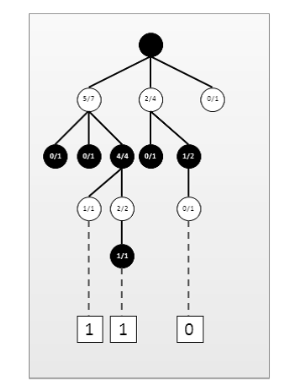
\includegraphics[keepaspectratio, scale=0.5,bb=0 0 304 387]
      {img/UCB.png}
 \caption{和了率評価を用いたモンテカルロ木探索}
 \label{monte2}
\end{figure}

\subsection{1人麻雀プレイヤにおける和了率の数理的評価}

国士氏の研究により、ある手牌における聴牌までの平均消費順目は、それぞれの変化での平均消費巡目のそれぞれの変化する確率での単純な平均で与えられることがわかっている。[3]すなわち、図\ref{kokusi}に示すように、元の成功率がp、手変わりする確率がq,r、手変わり後の成功率がQ,Rならば、

その手の向聴が進むまでの平均消費巡目は

\begin{equation}
\label{kitai1}
\Large \displaystyle \frac {p\frac{1}{p} + q\frac{1}{Q} + r\frac{1}{R}}{p+q+r}
\end{equation}

と表される。


変化の牌姿



この式\ref{kitai1}は、他プレイヤによって捨てられた牌を使ったシャンテン数現象パターン、すなわち鳴きを考慮していない。したがって面前聴牌のみを考えた式ということになる。しかし、1人麻雀においては相手プレイヤを考慮しないため、1人麻雀における聴牌率は4人麻雀における面前聴牌確率と一致し、この式によって求まる。鳴きによって聴牌する有効牌については、全て面前ツモで聴牌する有効牌の一部であり、制限によって鳴くことが出来ない有効牌も多く存在する。例えば、以下のような牌姿の場合である。


ヘッドレスイーシャンテンの牌姿を見て解説
図


また、面前聴牌と鳴きによる聴牌の違いについては、麻雀の役の性質上、和了することができなくなる制約や、点数が下がるなどの問題がある。したがって、鳴くことによる聴牌が面前聴牌に与える影響は少ないと考えられる。

ここで、本論文ではこれを和了時までの式に拡張する。

まず平均の関係から

\begin{figure}
 \centering
 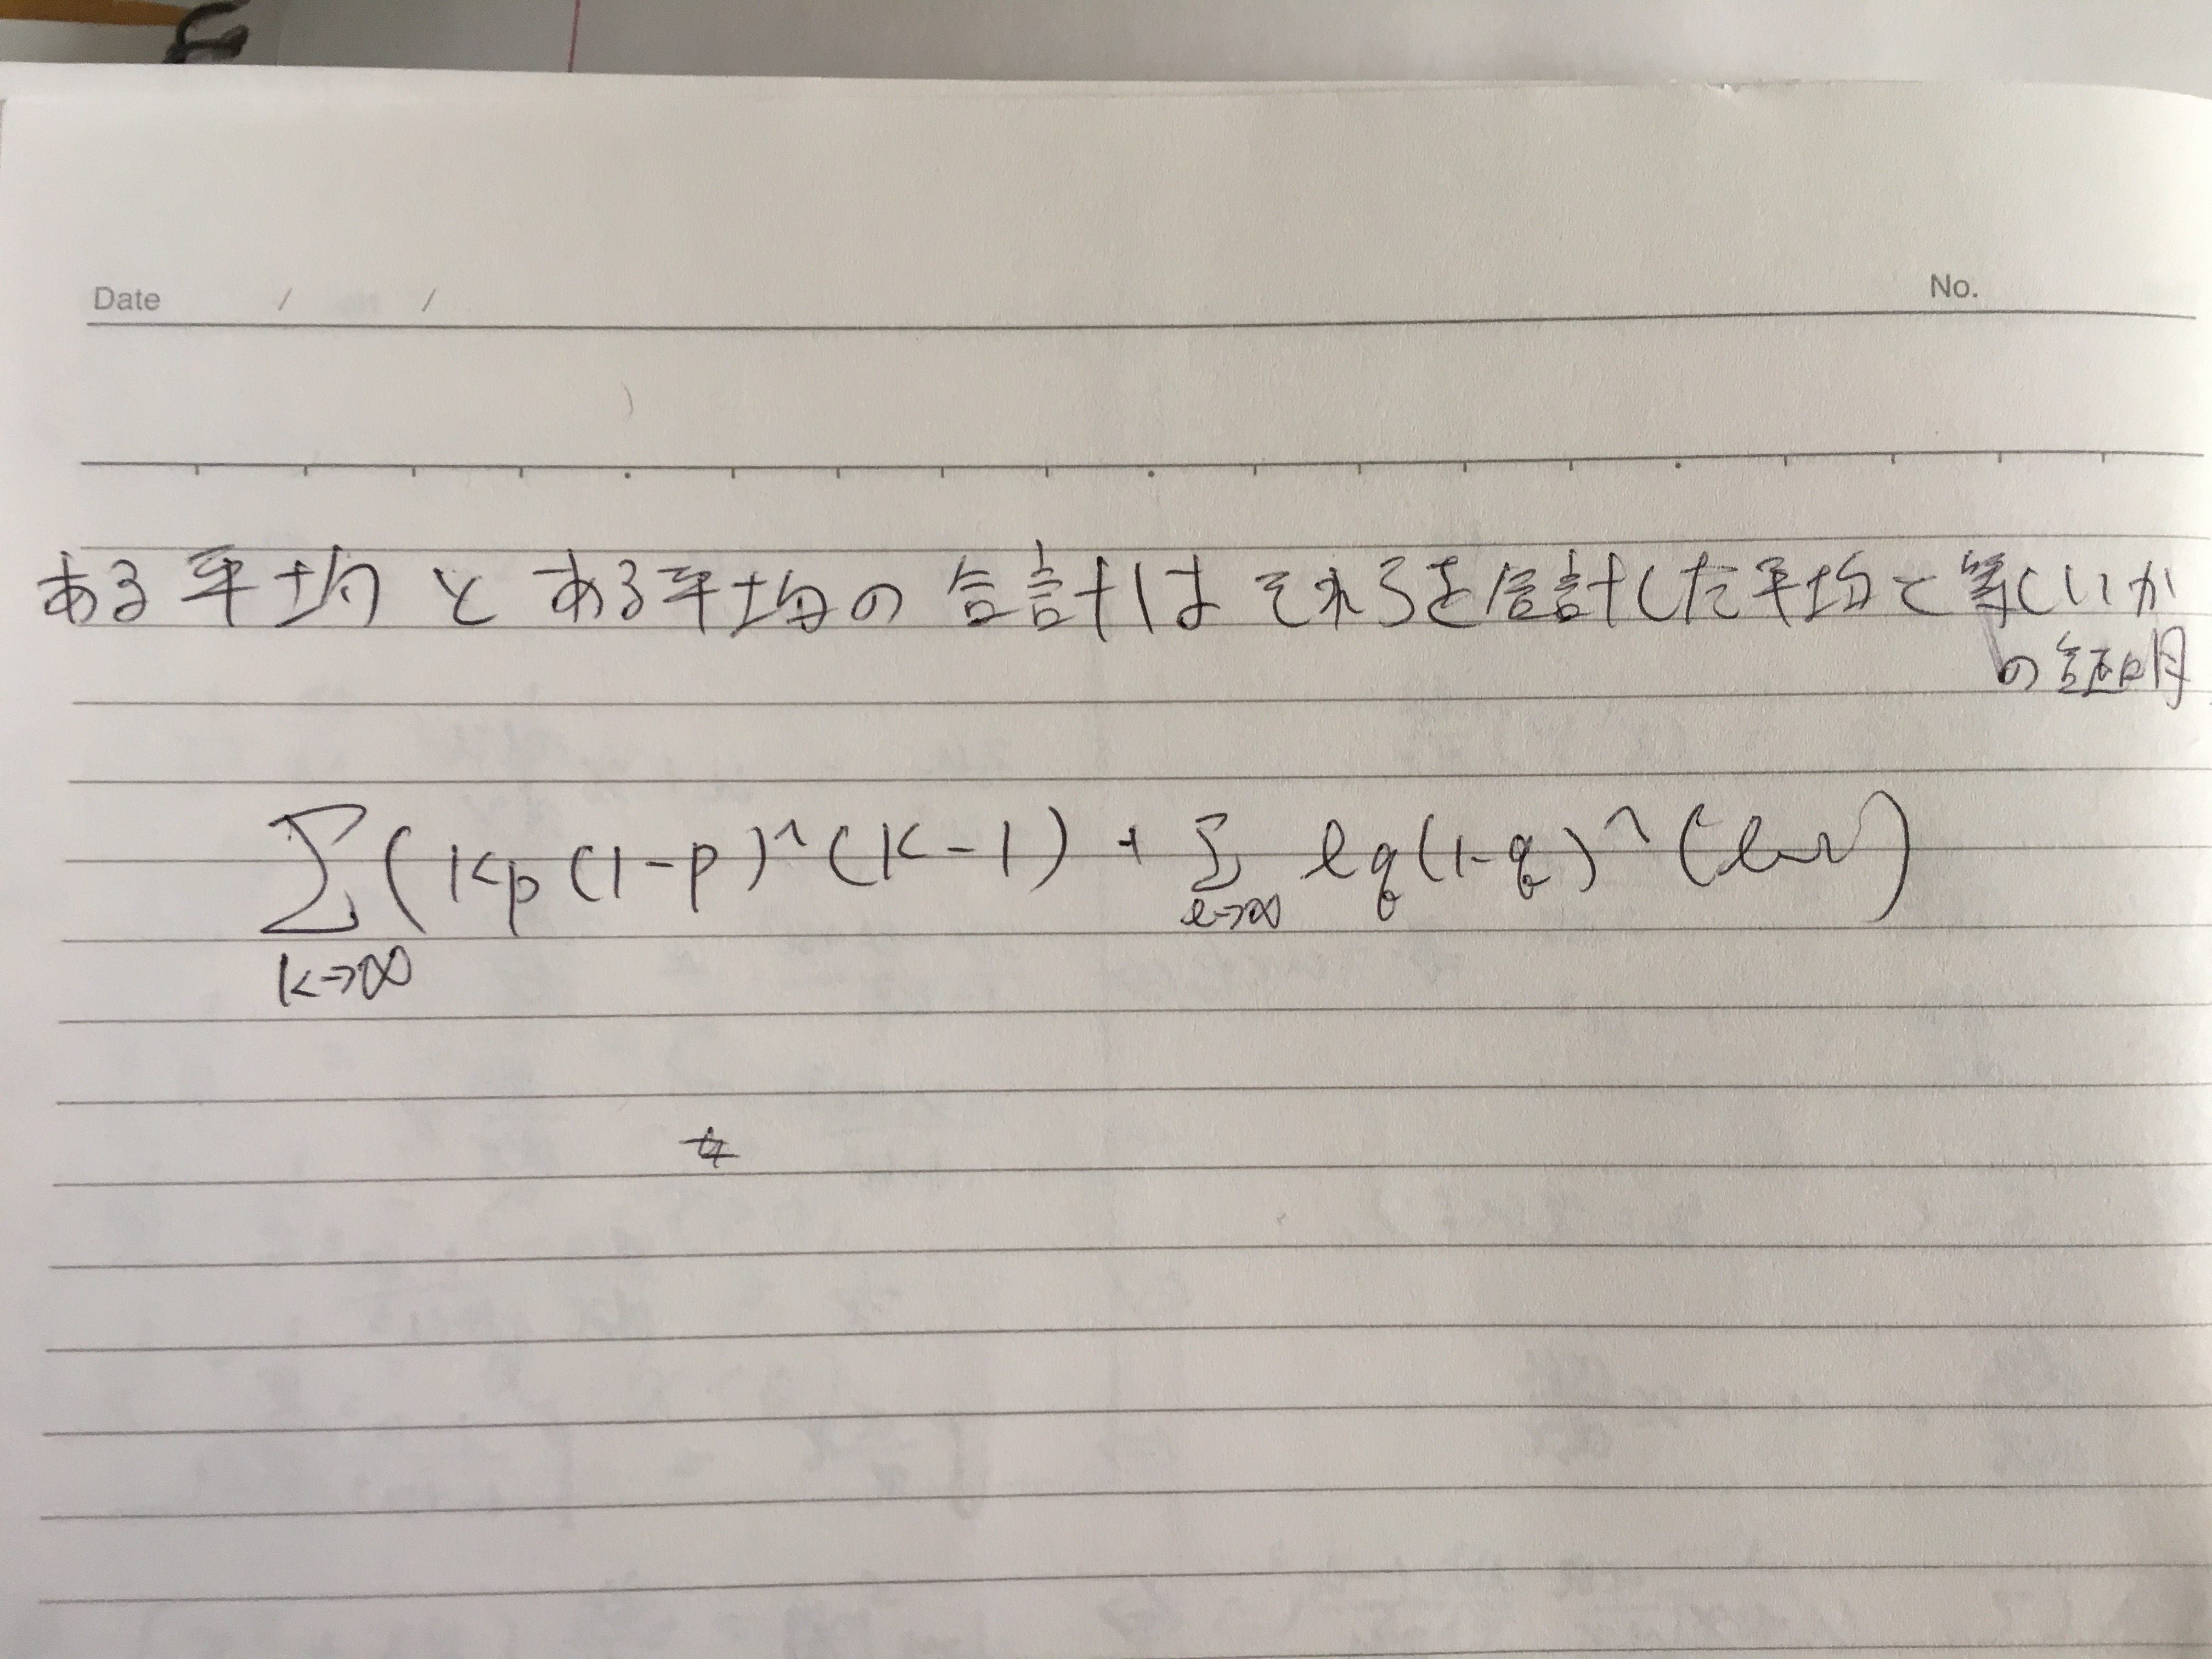
\includegraphics[keepaspectratio, scale=0.1,bb=0 0 4032 3024]
      {img/math.jpg}
 \caption{}
 \label{math}
\end{figure}

\begin{equation}
\label{kitai2}
\Large \displaystyle \frac {p\frac{1}{p} + q\frac{1}{Q} + r\frac{1}{R}}{p+q+r}
\end{equation}


ここで和了期待順目について考える


前節と同様に、4人麻雀において聴牌した

面前で聴牌するための平均消費順目と鳴きを考慮

まず、聴牌までの平均順目と聴牌後の和了までの平均順目の合計がすなわち全体の平均消費順目であることを証明する。
次に、それを合成した結果の数式がどうなるかを書く。

考察の結果このようになる。

\begin{equation}
\label{kitai2}
\Large \displaystyle \frac {p\frac{1}{p} + q\frac{1}{Q} + r\frac{1}{R}}{p+q+r} + 和了期待順目
\end{equation}
また、(現在の平均テンパイ巡目)=(次巡の平均テンパイ巡目)+1 であることから、
各ノードが手替わり率とテンパイ率を値として持つ深さ1の木構造で記述できる。 
したがって、同様に、n手先の手替わりまで考えると深さnの木構造で記述することができる。
nを大きくすることにより、精度の高い和了率を近似することが可能となる。

\begin{figure}
 \centering
 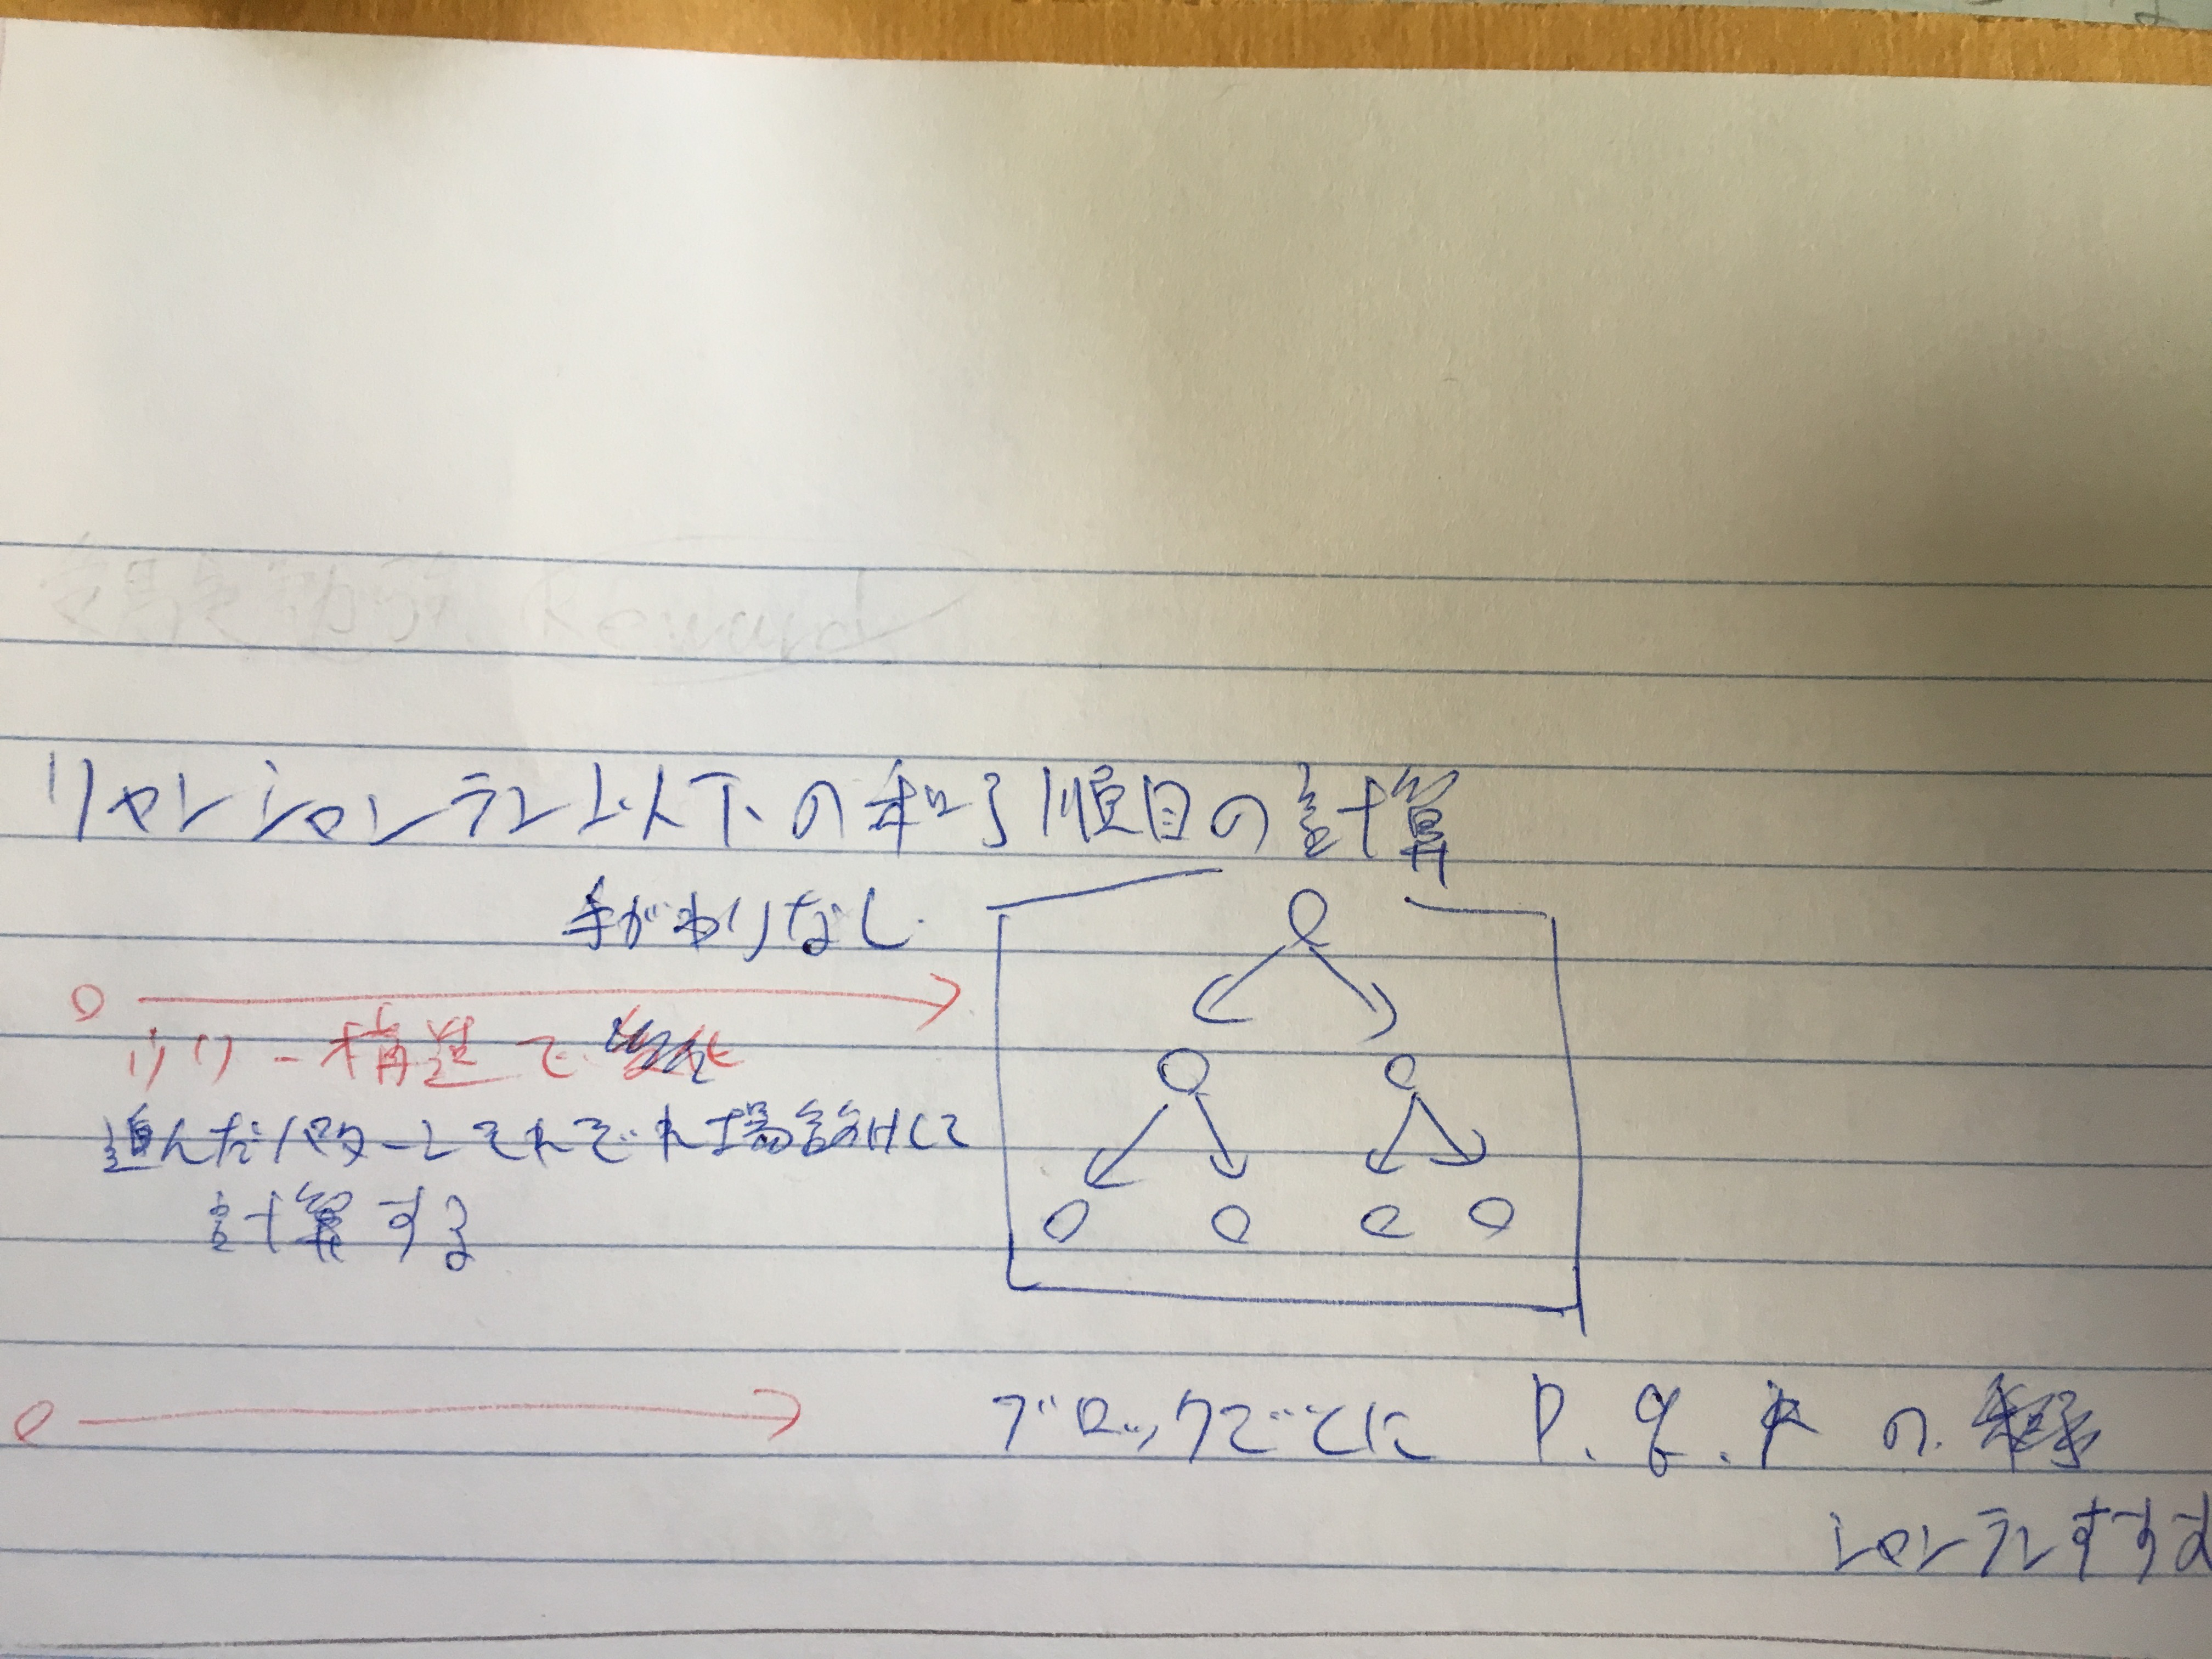
\includegraphics[keepaspectratio, scale=0.1,bb=0 0 4032 3024]
      {img/pqr.jpg}
 \caption{}
 \label{math}
\end{figure}

\begin{figure}
 \centering
 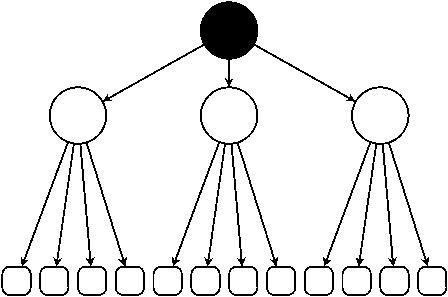
\includegraphics[keepaspectratio, scale=0.5,bb=0 0 500 281]
      {img/monte.jpg}
 \caption{図の説明}
 \label{ラベル名}
\end{figure}

本研究では、この式(3)をそれぞれの牌姿に当てはめ、その計算結果が高くなるようなノードを探索する。
これにより、従来の手法では何回も同じ牌姿の変化をシミュレートしなければいけない問題があったが、(3)式の評価によってその多くが削減できる。
したがって、この方法によって精度が高くなることが期待される。

\subsection{プレイアウトと平均報酬}

\begin{figure}
 \centering
 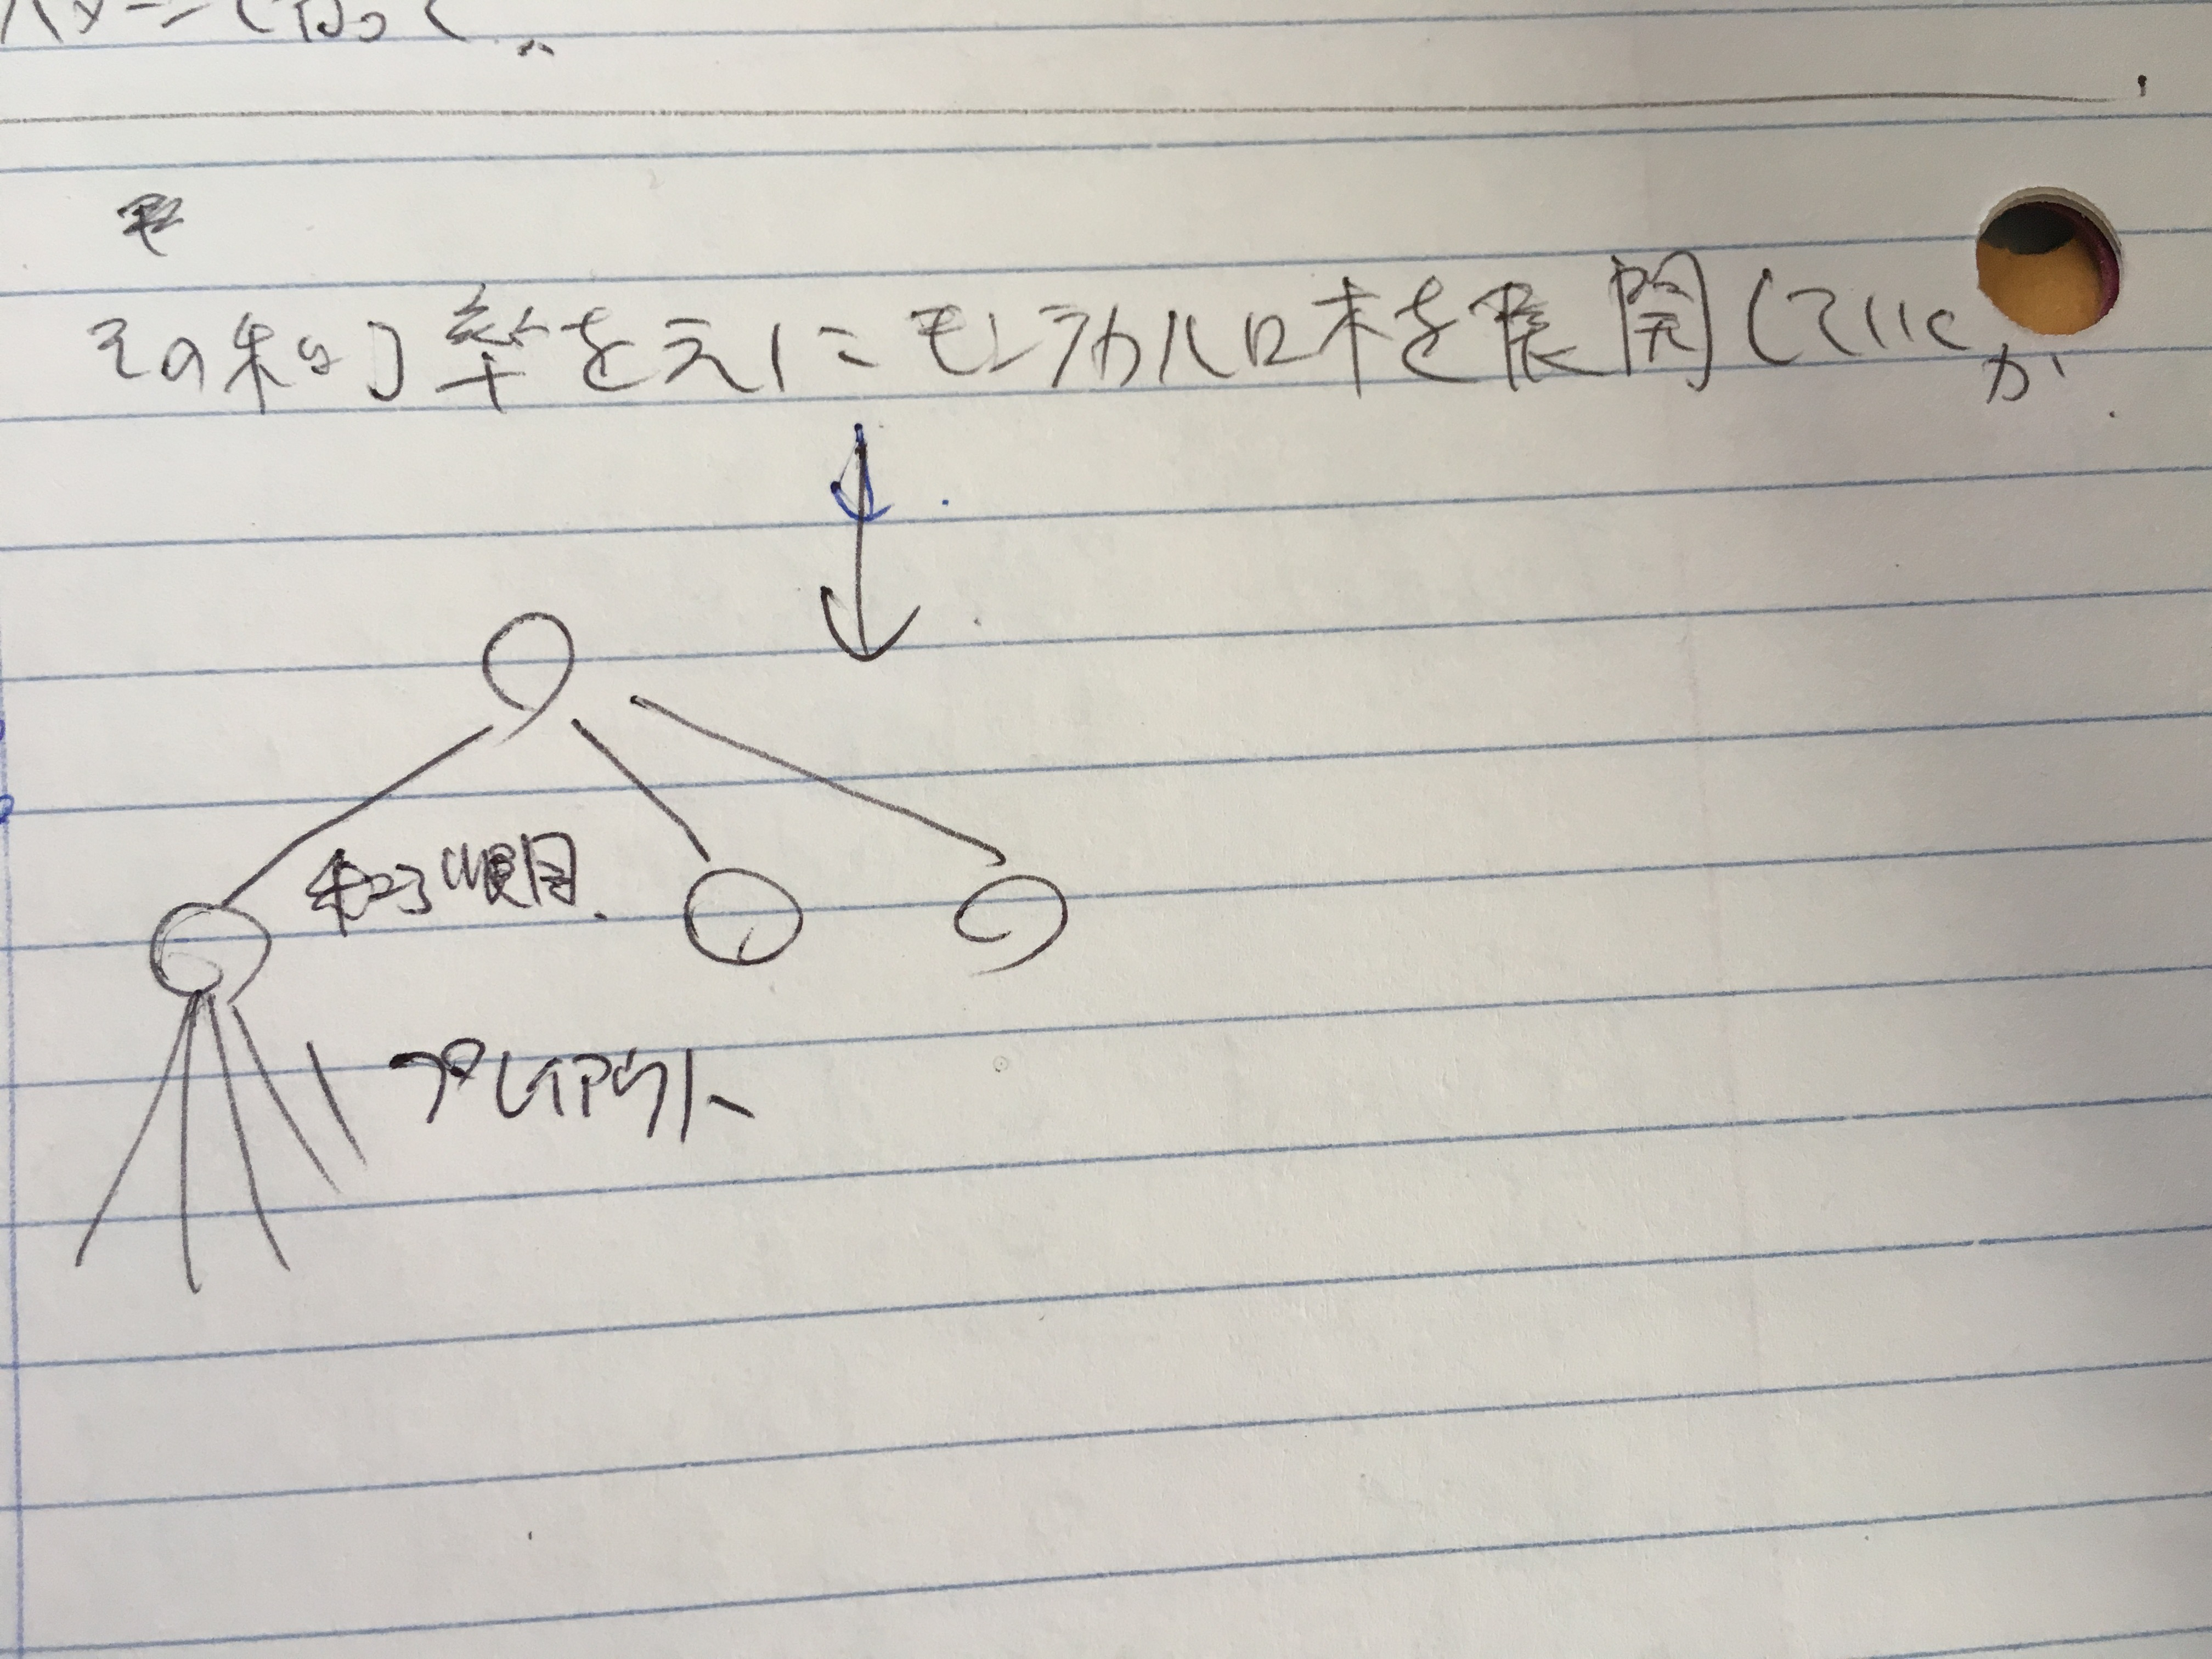
\includegraphics[keepaspectratio, scale=0.1,bb=0 0 4032 3024]
      {img/playout.jpg}
 \caption{}
 \label{math}
\end{figure}

普通に展開した場合は平均報酬と平均和了順目の関連性がないので、そこが問題。
単純に平均和了順目で比較するか、そもそも平均和了順目を報酬とすることで書き換えていくか。

% \subsection{二向聴以下の牌姿に対してモンテカルロ法を適用する}

% 麻雀において、和了までの手順の中では、シャンテン数が小さい時点での選択が成績に影響を与えやすいことがわかっている\cite{gendai}
% したがって、成績向上のためには和了系に近い部分において戦略を改善することが成績に影響を与えやすい事がわかる。

% また、モンテカルロ法の問題点は、前述したとおり麻雀に適用すると探索空間が大きくなりすぎることが問題であった。しかしこれを和了系に近い部分に適用することで、
% 探索空間を小さく削減することができるため、適用することができるようになる。
% 本研究の手法である与えられた牌姿における和了率の近似式(3)を適用する際にも、シャンテン数が大きすぎる場合については正確に見積もることが難しいため、このような限定的な部分への適用が重要である。

% 本論文では二向聴以上の部分にこのモンテカルロ法を適用することで、従来の問題点を解決する。
